\section{Development process}

\begin{frame}
    \frametitle{Development process}

    \begin{enumerate}
        \item \footnotesize Select building target.
            \begin{itemize}
                \item \scriptsize Binary
                \item \scriptsize Library: static (\texttt{*.o}) and shared (\texttt{*.so})
                \item \scriptsize Archive of library (\texttt{*.a})
                \item \scriptsize Libtool library (\texttt{*.la})
            \end{itemize}
        \item \footnotesize Project positioning.
            \begin{itemize}
                \item \scriptsize Multi-platform support (like CPU architectures, available resouorces)
                \item \scriptsize Embedded platform
                \item \scriptsize Library dependency and availability
                \item \scriptsize Distribution method (like APT, SourceForge, GitHub, binary, source code)
            \end{itemize}
        \item \footnotesize Code in \textit{C}.
        \item \footnotesize Build with compiler. (compile, link, $\cdots$)
            \begin{itemize}
                \item \scriptsize Language standards (like \textit{C99})
                \item \scriptsize Flags (like \texttt{-Wall})
                \item \scriptsize Dependent library headers
                \item \scriptsize Dependent library pre-compiled binary
                \item \scriptsize Code optimization (like \texttt{-O2 -O3})
                \item \scriptsize Debugging information
                \item \scriptsize Debug and profiling (like Valgrind, sanitizers, FlameGraph)
                    \begin{itemize}
                        \item \tiny Memory (heap) error (memory leak)
                        \item \tiny Thread error (racing)
                        \item \tiny Cache
                        \item \tiny Branch-prediction
                    \end{itemize}
            \end{itemize}
        \item \footnotesize Install, uninstall, system integration.
    \end{enumerate}
\end{frame}

\begin{frame}
    \frametitle{Deployment checks}

    How can we ensure that once the project is built, it can be executed correctly, consistently, and without problems?

    \begin{itemize}
        \item Pre-Build check list
            \begin{itemize}
                \item Compiler: \texttt{gcc}, \texttt{g++}, \texttt{clang}, \texttt{llvm}, $\cdots$
                \item Required software, library, function
                \item Version (like $>1.0.0$)
                \item Command execution location in project
            \end{itemize}
        \item Post-Build
            \begin{itemize}
                \item Can be executed or linked both locally and at the installing location
                \item Execution result is correct and consistent
            \end{itemize}
    \end{itemize}

    The thing is, coding \textit{C} is just a fraction of creating binaries and libraries.
\end{frame}

\begin{frame}
    \frametitle{Manual compile}
    
    % https://tex.stackexchange.com/questions/5818/how-to-center-a-listing

    If the project is not complicated, manually compiling everything or using a Bash script is acceptable. However, installing, uninstalling, and cleaning are not implemented.

    \begin{figure}[hp]
        \centering
        \hfill
        \begin{minipage}{.9\textwidth}
            \inputminted[
                mathescape,
                linenos,
                autogobble,
                fontsize=\scriptsize,
                firstline=2,
                lastline=4,
            ]{bash}{E:\\GitHub\\presentation_in_LaTeX\\c_project_development\\script\\term_cmd.sh}
        \end{minipage}
        \hfill
        \caption*{Commands for manual \texttt{gcc} compilation.}
    \end{figure}

    \begin{figure}[H]
        \centering
        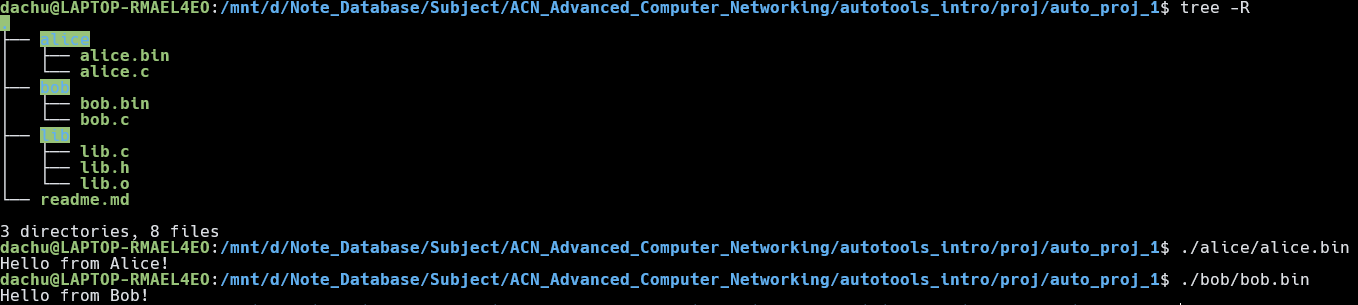
\includegraphics[width=0.9\textwidth]{../figure/manual_compile.png}
        \caption*{Tree structure and execution results after compilation.}
    \end{figure}
\end{frame}
